% ============================================================
% APPENDIX
% ============================================================
\appendix
\section*{Appendix}

% ----------------------------------------------------------
% Classical Thickness Distributions
% ----------------------------------------------------------

\subsection*{Cosine Spacing and Half-Cosine Spacing}

% ----- Motivation -----

\subsubsection*{Motivation}

In airfoil geometry discretization, 
a uniform spacing in the chordwise direction often fails to accurately capture regions with high curvature, especially near the leading edge. 
Since the leading edge radius is small and the curvature is large, 
clustering points in this region improves geometric resolution and numerical stability.

To achieve non-uniform but smoothly distributed points, 
cosine-based spacing techniques are commonly used.

% ----- Cosine Spacing -----

\subsubsection*{Cosine Spacing}

Let the chord length be normalized such that $x \in [0,1]$.  
The cosine spacing transformation is defined as:
\[
x(\theta) = \frac{1}{2}\left(1 - \cos \theta \right)
\quad \text{for } \theta \in [0,\pi]
\]

If $N$ points are required, we define:
\[
\theta_i = \frac{i\pi}{N-1}, \quad i = 0,1,\dots,N-1
\]

Thus,
\[
x_i = \frac{1}{2}\left(1 - \cos \frac{i\pi}{N-1} \right)
\]

Properties

\begin{itemize}
    \item Point clustering occurs near both $x=0$ (leading edge) and $x=1$ (trailing edge).
    \item The distribution is symmetric with respect to $x=0.5$.
    \item The spacing becomes denser near the endpoints.
\end{itemize}

% ----- Half-Cosine Spacing -----

\subsubsection*{Half-Cosine Spacing}

In some applications, clustering is only required near the leading edge.  
In this case, the half-cosine transformation is used:
\[
x(\theta) = 1 - \cos \theta 
\quad \text{for } \theta \in \left[0, \frac{\pi}{2}\right]
\]

For $N$ points:
\[
\theta_i = \frac{i}{N-1} \cdot \frac{\pi}{2}, \quad i = 0,1,\dots,N-1
\]

Thus,
\[
x_i = 1 - \cos \left( \frac{i}{N-1} \cdot \frac{\pi}{2} \right)
\]

Properties

\begin{itemize}
    \item Strong clustering near $x=0$.
    \item Nearly uniform spacing toward $x=1$.
    \item Particularly suitable for airfoil leading edge refinement.
\end{itemize}

% ----- Comparison with Uniform Spacing -----

\subsubsection*{Comparison with Uniform Spacing}

For reference, uniform spacing is defined as 
$
x_i = \displaystyle \frac{i}{N-1}
$

Uniform spacing does not account for geometric curvature and may require a significantly larger number of points to achieve comparable leading-edge accuracy. 
Cosine-based spacing provides higher geometric resolution with the same number of discretization points.

% ----------------------------------------------------------
% Classical Thickness Distributions
% ----------------------------------------------------------

\subsection*{Lagrange Interpolation}

% ----- Definition -----

\subsubsection*{Definition}

Given a set of $n+1$ distinct data points:
\[
(x_0, y_0), (x_1, y_1), \dots, (x_n, y_n)
\]

the Lagrange interpolation polynomial $P_n(x)$ of degree at most $n$ is defined as:
\[
P_n(x) = \sum_{j=0}^{n} y_j L_j(x)
\]

where $L_j(x)$ are the Lagrange basis polynomials:
\[
L_j(x) = \prod_{\substack{m=0 \\ m \ne j}}^{n}
\frac{x - x_m}{x_j - x_m}
\]

% ----- Interpolation Property ----- 

\subsubsection*{Interpolation Property}

The basis polynomials satisfy:
\[
L_j(x_i) =
\begin{cases}
1, & i=j \\
0, & i \ne j
\end{cases}
\]

Thus,
\[
P_n(x_i) = y_i
\]

which guarantees exact interpolation at the given nodes.

% ----- Application in Airfoil Geometry -----

\subsubsection*{Application in Airfoil Geometry}

In airfoil reconstruction, Lagrange interpolation can be used to:

\begin{itemize}
    \item Interpolate discrete airfoil coordinate data.
    \item Construct smooth curves from control points.
    \item Approximate camber line or thickness distribution functions.
\end{itemize}

However, for large $n$, high-degree interpolation may suffer from Runge's phenomenon, 
especially under uniform spacing. Using cosine-spaced nodes significantly improves numerical stability.

% ----- Error Estimation -----

\subsubsection*{Error Estimation}

The interpolation error is given by:
\[
f(x) - P_n(x) =
\frac{f^{(n+1)}(\xi)}{(n+1)!}
\prod_{i=0}^{n}(x - x_i)
\]

for some $\xi$ in the interval containing the nodes.

This expression shows that:
\begin{itemize}
    \item The error depends on node placement.
    \item Clustering nodes (e.g., cosine spacing) reduces oscillatory behavior.
\end{itemize}

% ----------------------------------------------------------
% Classical Thickness Distributions
% ----------------------------------------------------------

\subsection*{Representatives of Classical NACA Airfoils}
\centering
\begin{figure}[h!]
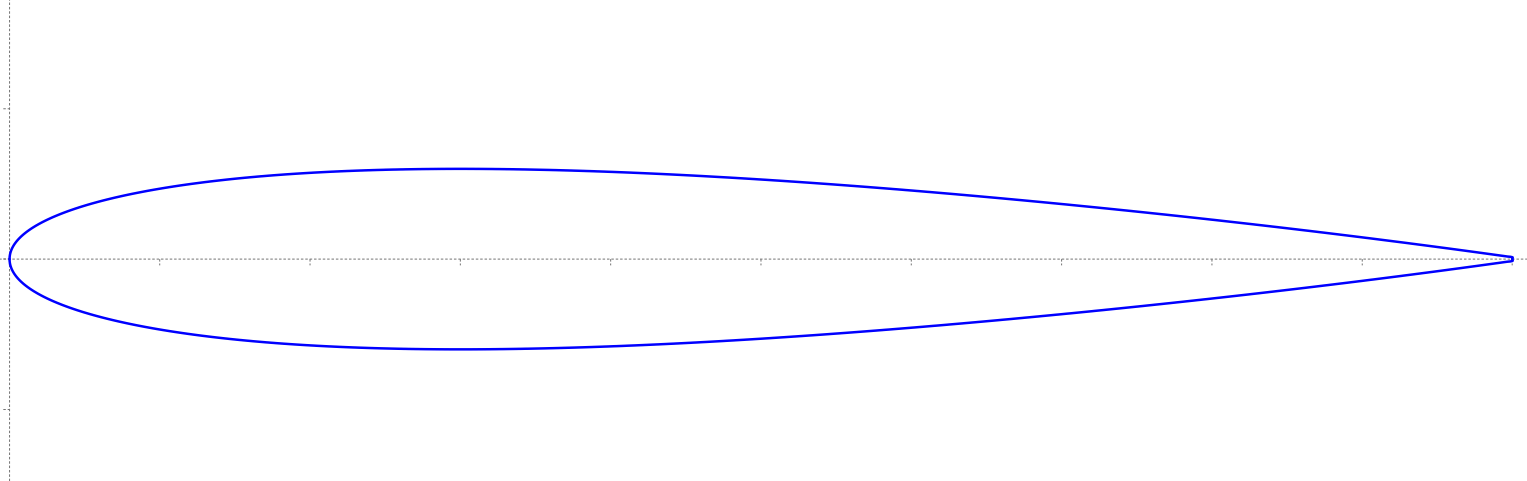
\includegraphics[width=1\textwidth]{figures/naca0012.png}
\caption{NACA 0012}
\end{figure}

\begin{figure}[h!]
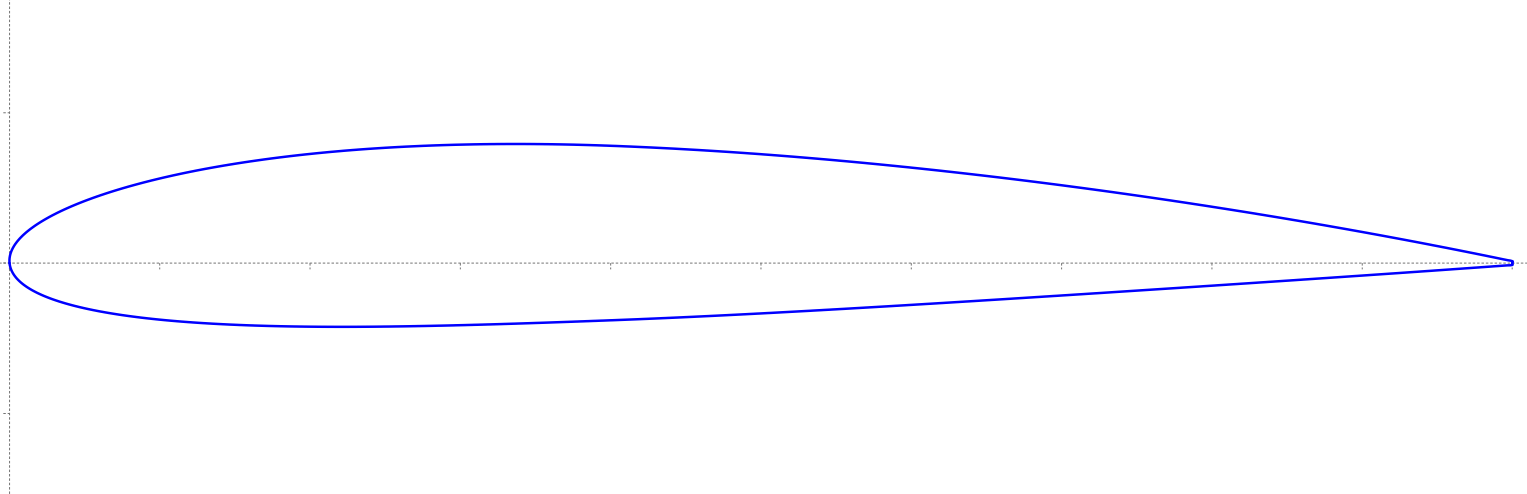
\includegraphics[width=1\textwidth]{figures/naca2412.png}
\caption{NACA 2412}
\end{figure}

\begin{figure}[h!]
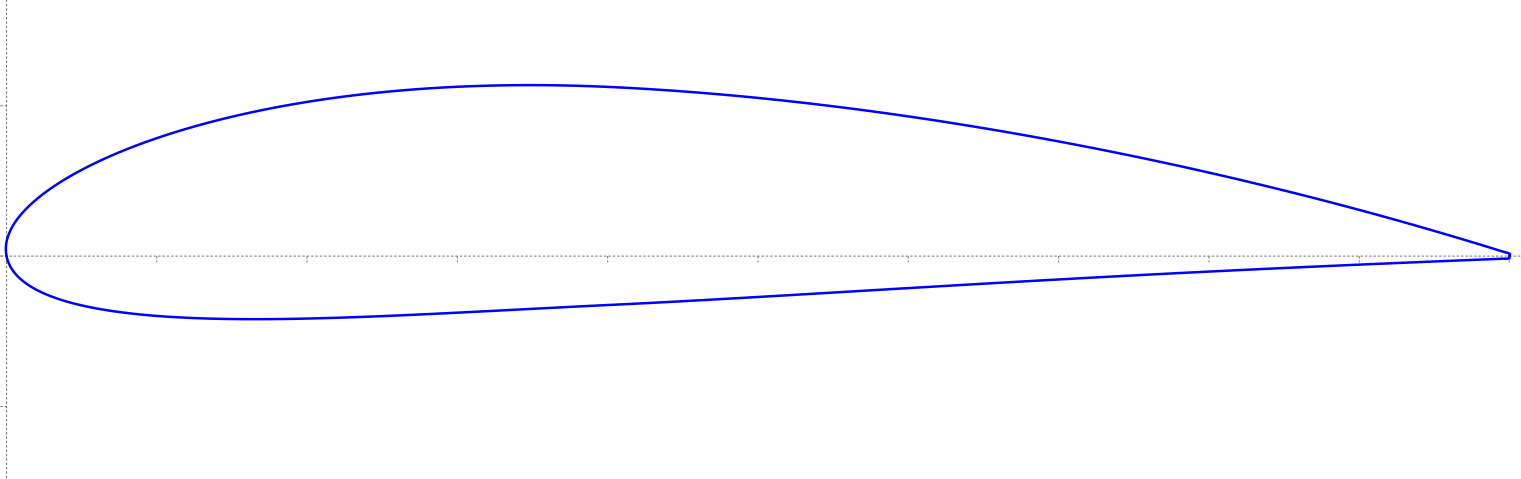
\includegraphics[width=1\textwidth]{figures/naca4415.png}
\caption{NACA 4415}
\end{figure}

\begin{figure}[h!]
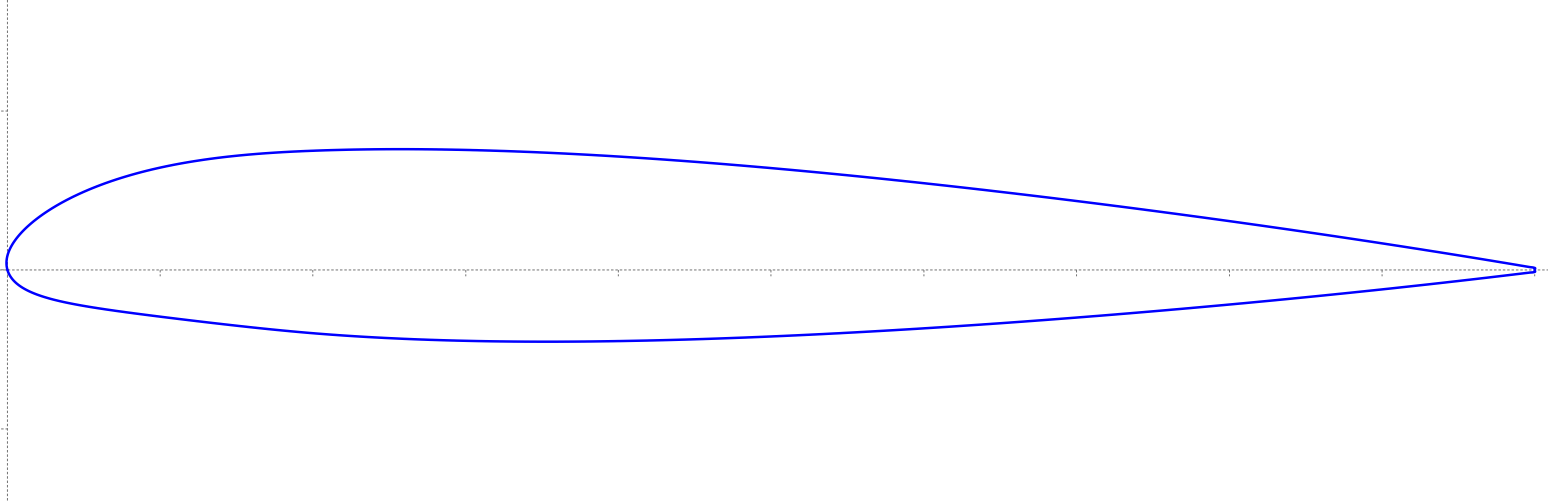
\includegraphics[width=1\textwidth]{figures/naca23012.png}
\caption{NACA 23012}
\end{figure}

\begin{figure}[h!]
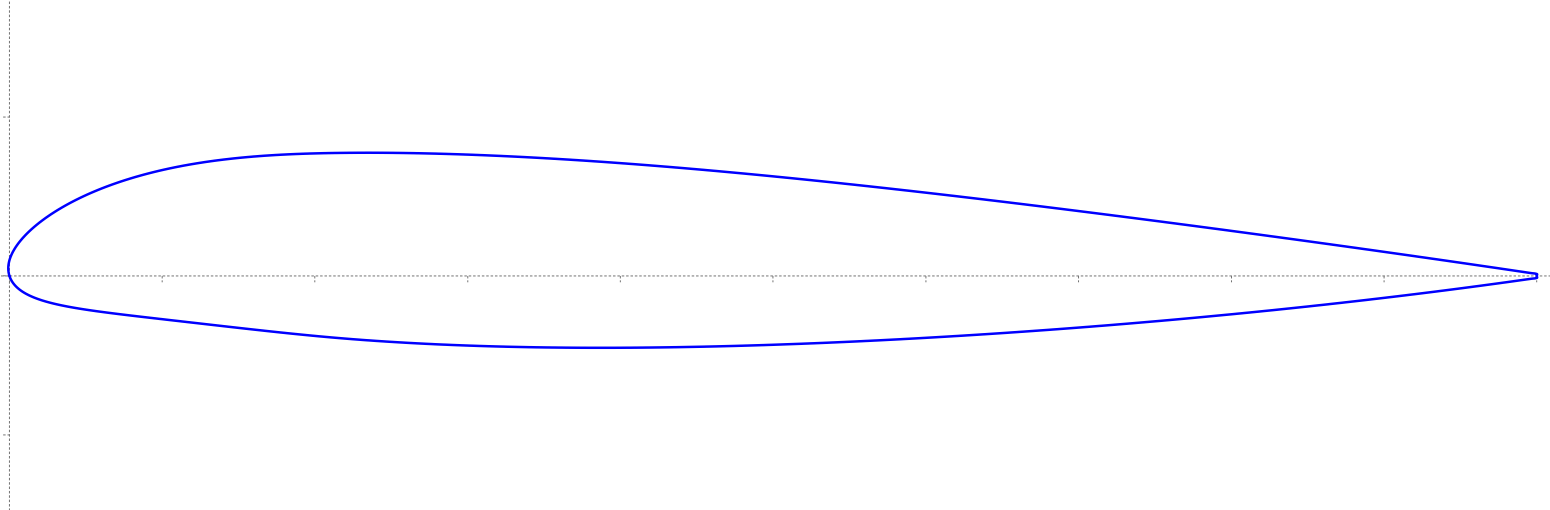
\includegraphics[width=1\textwidth]{figures/naca23112.png}
\caption{NACA 23112}
\end{figure}

\begin{figure}[h!]
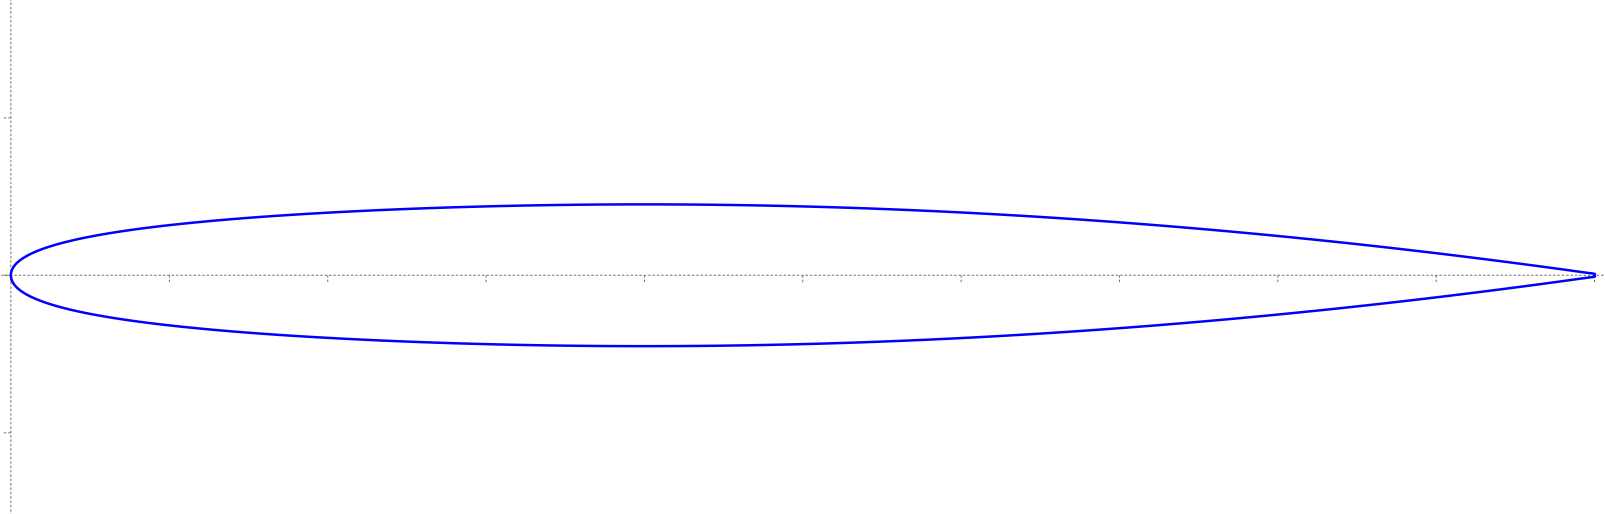
\includegraphics[width=1\textwidth]{figures/naca0009-64.png}
\caption{NACA 0009-64}
\end{figure}

\begin{figure}[h!]
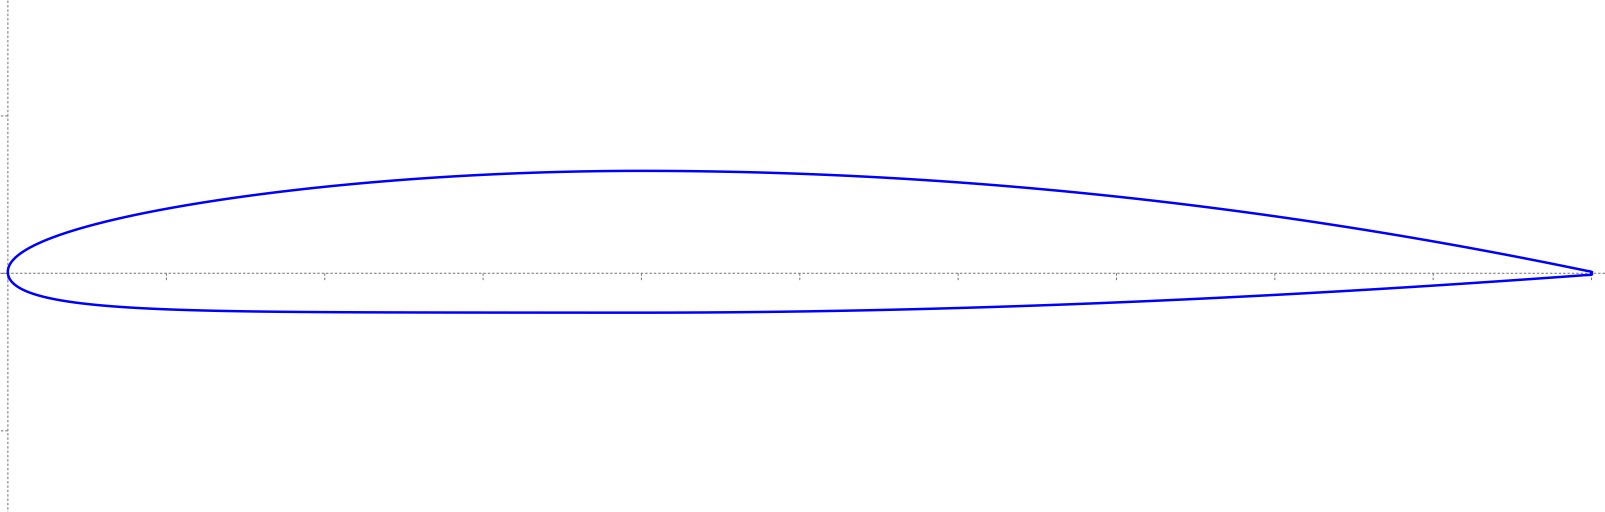
\includegraphics[width=1\textwidth]{figures/naca2409-64.png}
\caption{NACA 2409-64}
\end{figure}

\begin{figure}[h!]
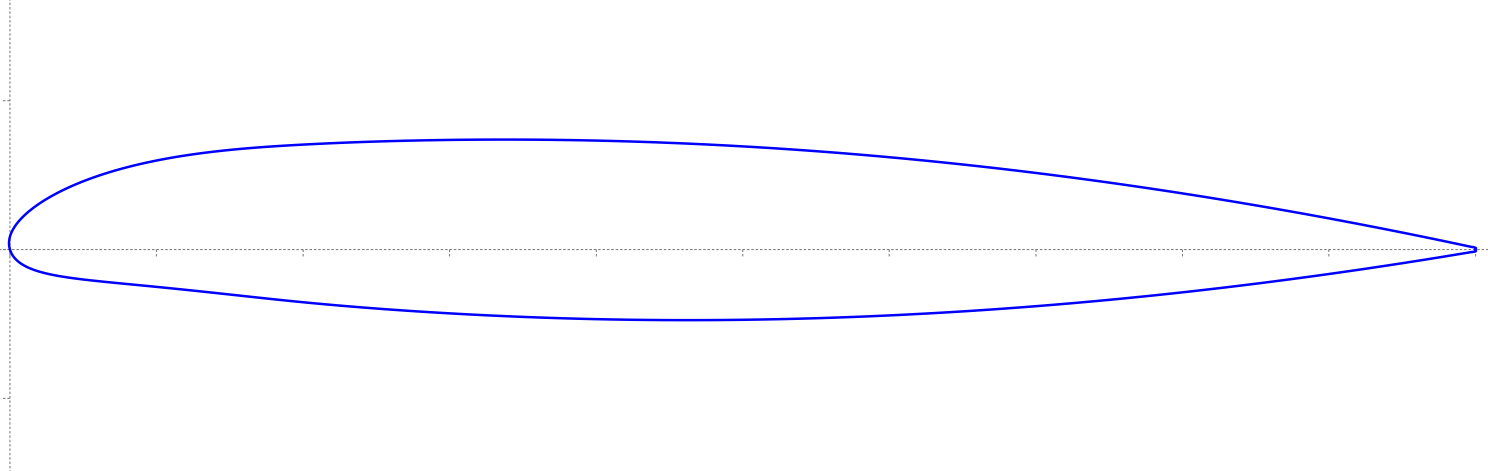
\includegraphics[width=1\textwidth]{figures/naca23012-64.png}
\caption{NACA 23012-64}
\end{figure}

\begin{figure}[h!]
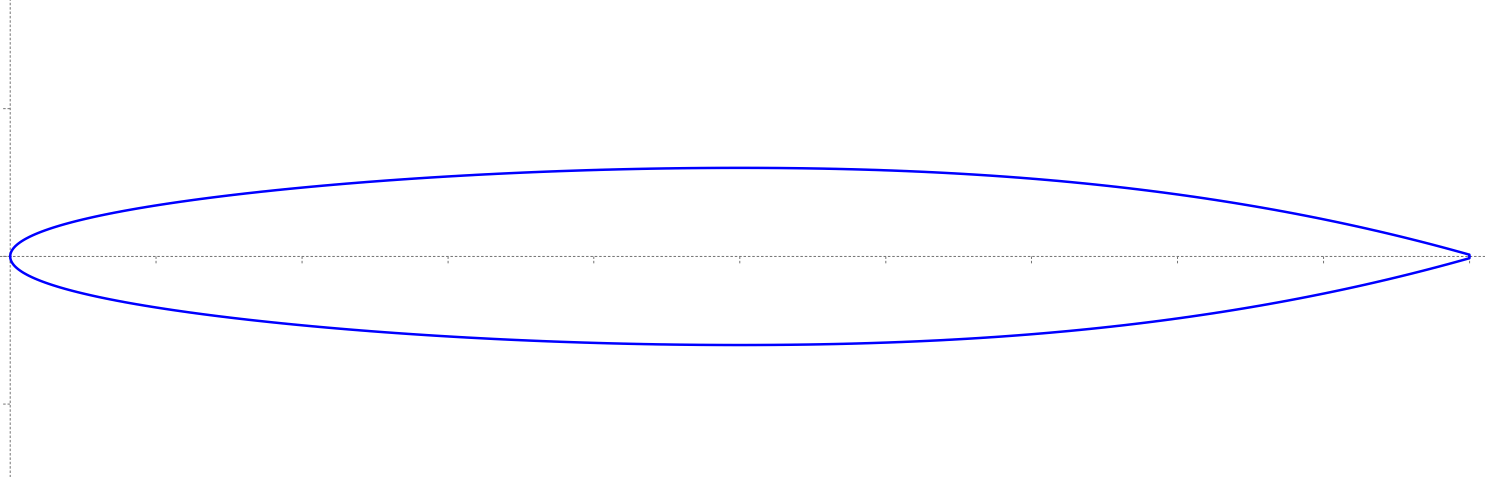
\includegraphics[width=1\textwidth]{figures/naca16-012.png}
\caption{NACA 16-012}
\end{figure}

\begin{figure}[h!]
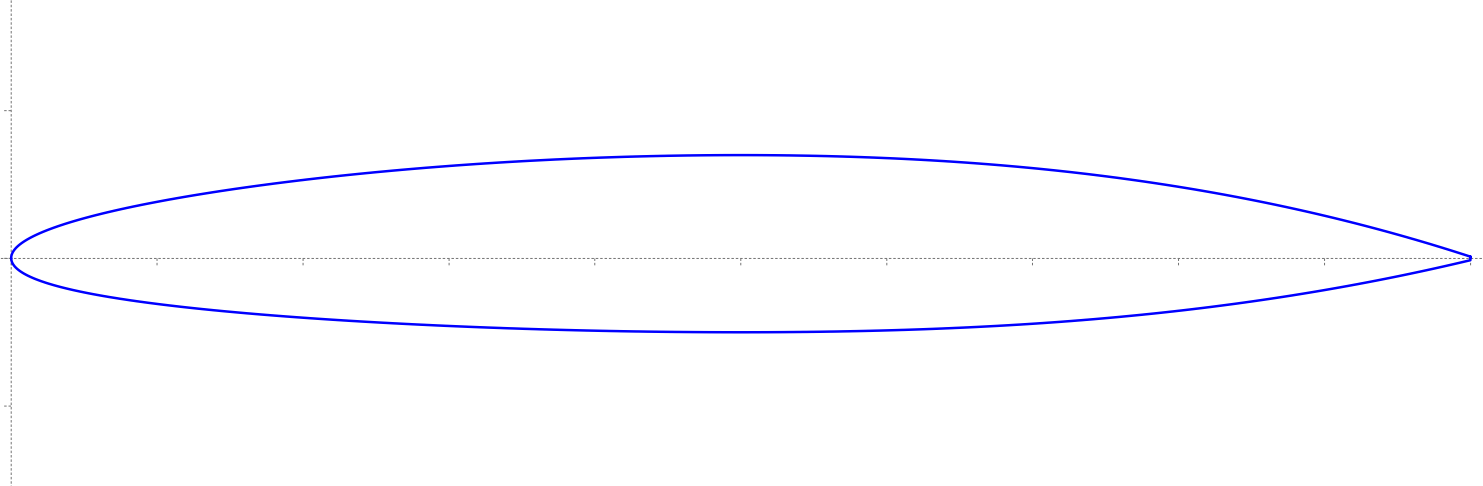
\includegraphics[width=1\textwidth]{figures/naca16-212.png}
\caption{NACA 16-212}
\end{figure}

\begin{figure}[h!]
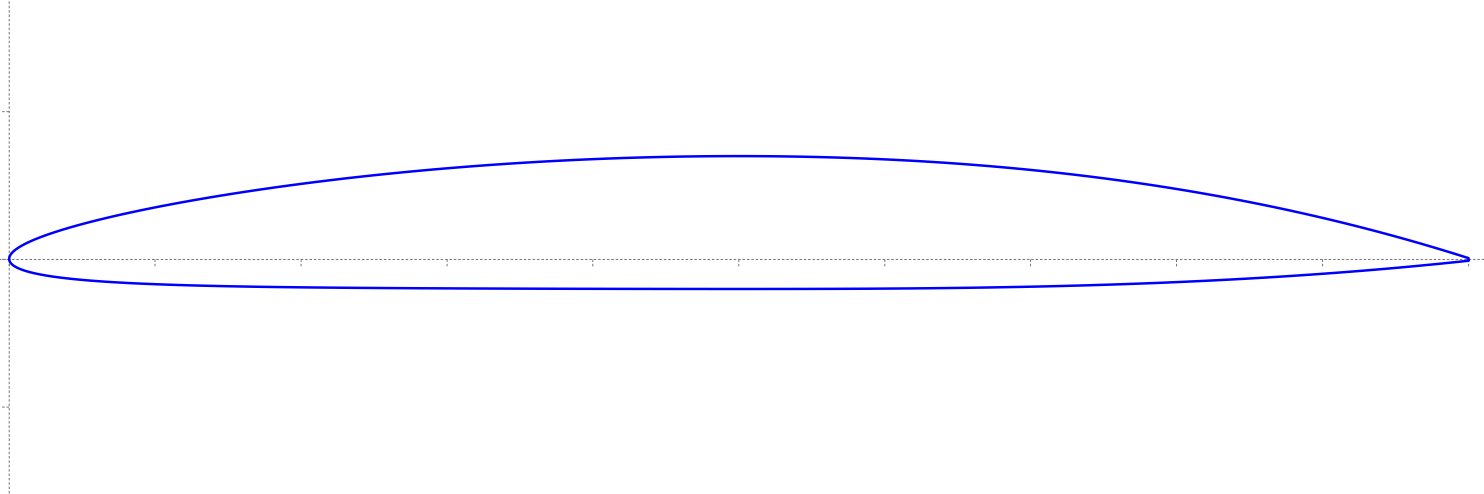
\includegraphics[width=1\textwidth]{figures/naca16-509.png}
\caption{NACA 16-509}
\end{figure}


